\documentclass{article}
\usepackage{tikz}
\usepackage{pgfplots}
\usepackage{svg}
\usepackage{amsmath}
\usepackage{array}
\usepackage[skins]{tcolorbox}
\usepackage[version=4]{mhchem}
\usepackage[a4paper, total={6in, 9in}]{geometry}
\usepackage{fourier}
\usepackage{xymtex}
\usepackage{textcomp}
\usepackage{eurosym}
\usepackage{caption}
\usepackage{longtable}
\usepackage{float}
\usepackage{attachfile}
\usepackage{multirow}
\usepackage{amsfonts} 
\usepackage{xcolor}
\usepackage{tabularray}
\UseTblrLibrary{booktabs}

\captionsetup[table]{name=Tabella}
\pagenumbering{gobble}
%\setcounter{secnumdepth}{2}

\definecolor{myblue}{RGB}{224, 245, 255} 
\definecolor{myred}{RGB}{234, 222, 255}
\definecolor{myorange}{RGB}{255, 102, 0}

\renewcommand*\contentsname{Indice}
\setcounter{tocdepth}{3}
\setcounter{secnumdepth}{2}
\pgfplotsset{compat=1.15}


\title{Relazione di laboratorio - Esperienza di Poisson}
\author{Federico Cesari}
\date{Marzo 2024}




\begin{document}
\begin{titlepage}
	\begin{center}
		\vspace*{1cm}
		
		\textbf{\LARGE Relazione di laboratorio - Pendolo semplice}
		
		\vspace{0.3cm}
		\large \textit{Misura del periodo di un pendolo semplice} \\
		
		\vspace{0.5cm}
		\Large Federico Cesari \\
		
		\small 1096759 
		\vspace{0.2cm}
		
		\small Gruppo 5
		
		
		\vspace{3cm}
		\begin{center}
			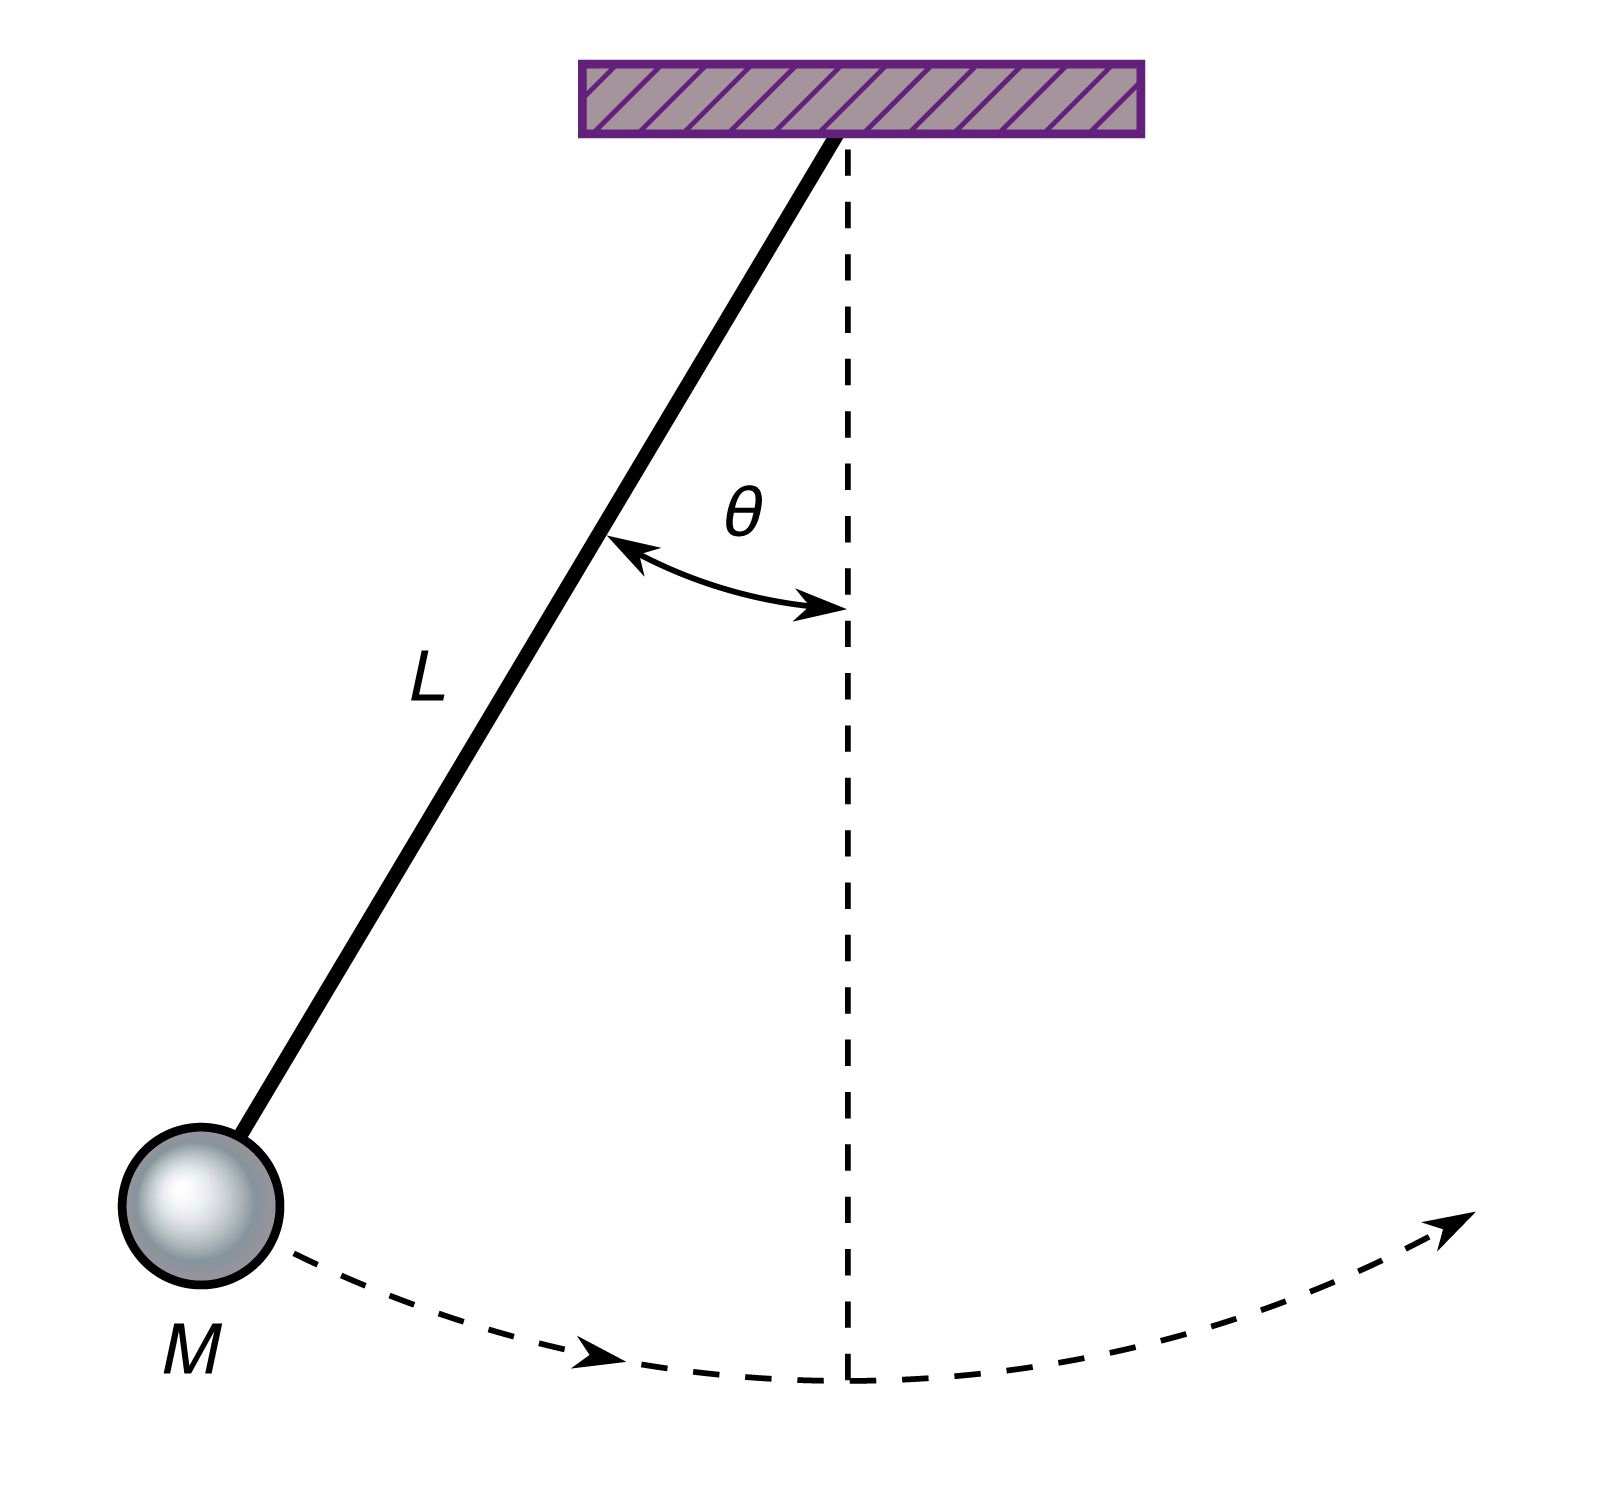
\includegraphics[scale=0.1]{IMG_0200.jpeg}	
		\end{center}
		
		
		
		\vfill
		
		
		
		corso A\\
		Università degli studi di Torino, Torino\\
		4 aprile 2024\\
		
		
	\end{center}
\end{titlepage}
\tableofcontents

\newpage
\textcolor{white}{.}
\vfill


\section{Scopo dell’esperienza}
\section{Premesse teoriche}
\section{Scelta strumento di misura}

Al fine di stabilire il migliore strumento di misura per le succesive analisi dati, prendo 8 misure del periodo del pendolo prima con un angolo di partenza $\vartheta = 5^\circ$ e poi con $\vartheta = 30^\circ$.



\begin{table}[H]
	\label{tab:example}
	\caption{\textit{Confronto strumenti di misura}}
	\centering
	\begin{tblr}{
			colspec={c|ccc},
			row{1}={font=\bfseries},
			row{2}={bg=white},
			column{1}={font=\itshape},
		}
		\toprule
		& Cronometro analogico & Cronometro digitale &  Fotocellula  \\
		$\vartheta \pm 1^\circ $& $T(s) \pm 0.2s$      & $T(s) \pm 0.01s$     & $T(s) \pm 0.001s$   \\
		\toprule
		\SetCell[r=4]{c} $5^\circ$ & 1.7 & 1.63 & 1.706  \\ \hline[dashed] 
									& 1.6 & 1.59 & 1.706  \\ \hline[dashed] 
								 	& 1.7 & 1.50 & 1.706  \\ \hline[dashed]
									& 1.7 & 1.60 & 1.706  \\ 
		
									\hline 
		\SetCell[r=4]{c} $30^\circ$ & 1.8 & 1.65 & 1.715  \\ \hline[dashed]
								 	& 1.7 & 1.71 & 1.715  \\ \hline[dashed]
								 	& 1.6 & 1.70 & 1.716  \\ \hline[dashed]
								 	& 1.7 & 1.66 & 1.715  \\ 
		\bottomrule
	\end{tblr}
\end{table}


\begin{table}[H]
	\label{tab:example}
	\caption{\textit{Periodi medi}}
	\centering
	\begin{tblr}{
			colspec={c|ccc},
			row{1}={font=\bfseries},
			row{2}={bg=white},
			column{1}={font=\itshape},
		}
		\toprule
		& Cronometro analogico & Cronometro digitale &  Fotocellula  \\
		$\vartheta \pm 1^\circ $& $\bar{T}(s) \pm 0.05s$      & $\bar{T}(s) \pm 0.005s$     & $\bar{T}(s) \pm 0.0005s$   \\
		\toprule
		 $5^\circ$ & $1.65$ & $1.700$  & $1.7060$  \\
		\hline 
		 $30^\circ$ & $1.70$ & $1.680$ & $1.7150$  \\ 
		\bottomrule
	\end{tblr}
\end{table}



\section{Dipendenza dall’angolo}

\begin{figure}[H]
	\centering
	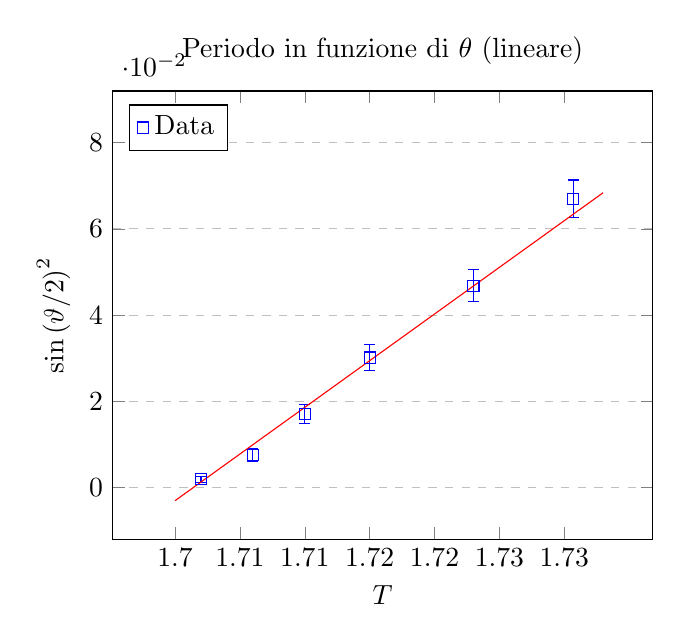
\begin{tikzpicture}
		\begin{axis}[
			title={Periodo in funzione di $\theta$ (lineare)},
			xlabel={$T$},
			ylabel={$\sin{\left( \vartheta / 2\right) }^2$},
			xmin=1.7, xmax=1.732,
			ymin=0, ymax=0.08,
			xtick={1.7,1.705,1.71,1.715,1.72,1.725,1.73},
			ytick={0,0.02,0.04,0.06,0.08},
			legend pos=north west,
			ymajorgrids=true,
			grid style=dashed,
			enlargelimits=0.15,
			]
			
			\addplot[
			only marks,
			color=blue,
			mark=square,
			error bars/.cd,
			y dir=both, y explicit
			]
			coordinates {
				(1.702,0.0019027) +- (0,0.00075825)
				(1.706,0.0075961) +- (0,0.00151074)
				(1.710,0.0170371) +- (0,0.00225173)
				(1.715,0.0301537) +- (0,0.00297558)
				(1.723,0.0468461) +- (0,0.00367678)
				(1.7307,0.0669873) +- (0,0.00435)
			};
			\addplot[
				domain=1.7:1.733, 
				samples=100, 
				color=red, 
				] 
				{2.16490*x -3.68337};
			\legend{Data}
		\end{axis}
	\end{tikzpicture}
	\caption{$T\left( \sin{\left( \vartheta / 2\right) }^2\right) $}
\end{figure}


\begin{figure}[H]
	\centering
	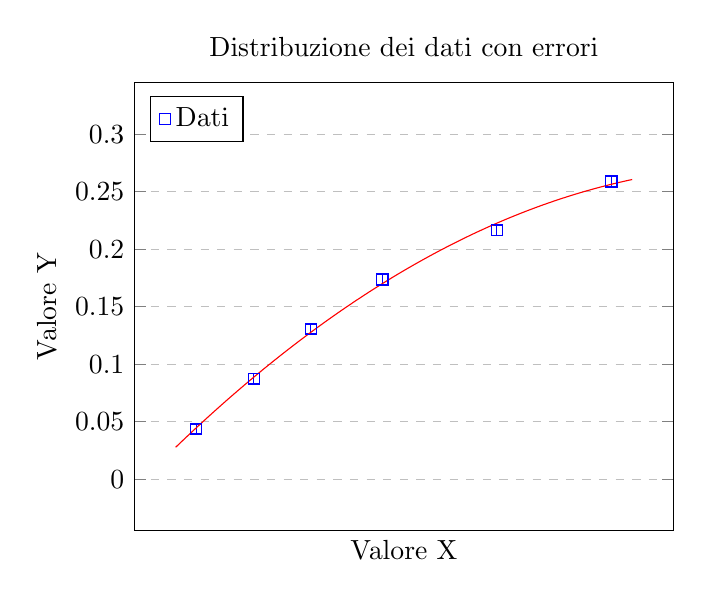
\begin{tikzpicture}
		\begin{axis}[
			title={Distribuzione dei dati con errori},
			xlabel={Valore X},
			ylabel={Valore Y},
			xmin=-1, xmax=1,
			ymin=0, ymax=0.3,
			xtick={1.7,1.71,1.72,1.73,1.74},
			ytick={0,0.05,0.1,0.15,0.2,0.25,0.3},
			tick label style={/pgf/number format/fixed},
			legend pos=north west,
			ymajorgrids=true,
			grid style=dashed,
			enlargelimits=0.15,
			]
			
			\addplot[
			only marks,
			mark=square,
			color=blue,
			error bars/.cd,
			y dir=both, y explicit
			]
			coordinates {
				(-1,0.0436194) +- (0,0.0086917/2)
				(-0.7241,0.0871557) +- (0,0.0086669/2)
				(-0.4482,0.1305262) +- (0,0.0086256/2)
				(-0.10344,0.1736482) +- (0,0.0085678/2)
				(0.4482,0.2164396) +- (0,0.0084938/2)
				(1,0.2588190) +- (0,0.0084036/2)
			};
			\addplot[
			domain=-1.1:1.1, 
			samples=100, 
			color=red, 
			] 
			{-0.03080*x^2 + 0.105900*x + 0.18138};
			\legend{Dati}
		\end{axis}
	\end{tikzpicture}
	\caption{Rappresentazione grafica dei dati sperimentali con errori ridotti.}
\end{figure}

\subsection{Confronto parametri parabola}

\subsection{g}

Calcolo il valore di g:
\[
T_0 = 2\pi\sqrt{\frac{l}{g}} \qquad \to \qquad T_0^2 = 4\pi^2\frac{l}{g}
\] 
\[
g = \frac{4l\pi^2}{T_0^2}
\]

poiché sappiamo che

\[
T = T_0 + \frac{T_0}{4}y \qquad \to \qquad y = 4\frac{T-T_0}{T_0} \qquad \to \qquad y = 4\frac{T}{T_0} - 4
\]
\[
b = \frac{4}{T_0} \qquad \to \qquad T_0 = \frac{4}{b}
\]

Quindi

\[
\mathbf{g = \frac{l\pi^2}{4}b^2}
\]

Calcolo l'errore associato a g:
\[
\sigma_g = \sqrt{\left(\frac{\partial g}{\partial l} \right)^2\sigma_l^2 + \left(\frac{\partial g}{\partial b} \right)^2 \sigma_b^2}
\]
\[
\sigma_g = 	\sqrt{\left(\frac{b^2\pi^2}{4}\right)^2 \sigma_l^2 + \left( \frac{lb\pi^2}{2}  \right)^2 \sigma_b^2	 }
\]

\subsubsection{Test Z per g}

Ottengo $g = ...$ ... Scelgo livello di significatività = 0.05.



\section{Dipendenza dalla lunghezza}

\begin{figure}[H]
	\centering
	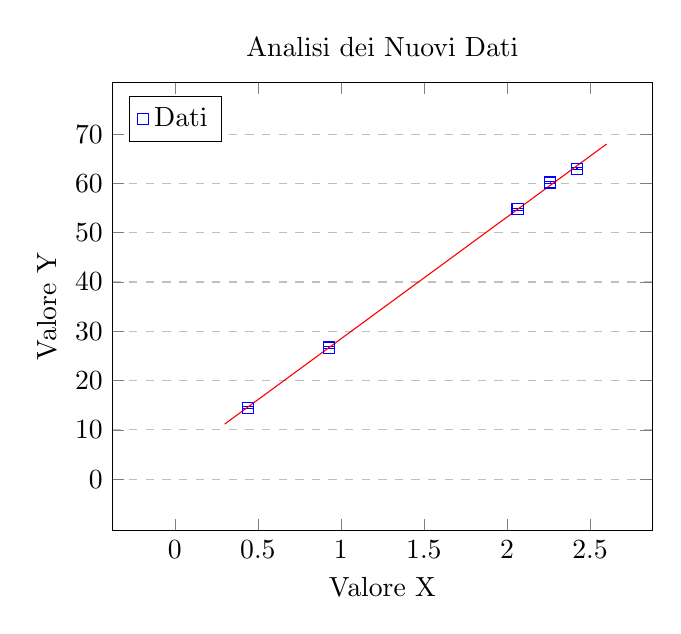
\begin{tikzpicture}
		\begin{axis}[
			title={Analisi dei Nuovi Dati},
			xlabel={Valore X},
			ylabel={Valore Y},
			xmin=0, xmax=2.5,
			ymin=0, ymax=70,
			xtick={0,0.5,1,1.5,2,2.5},
			ytick={0,10,20,30,40,50,60,70},
			legend pos=north west,
			ymajorgrids=true,
			grid style=dashed,
			enlargelimits=0.15,
			]
			
			\addplot[
			only marks,
			color=blue,
			mark=square,
			error bars/.cd,
			y dir=both, y explicit
			]
			coordinates {
				(2.260011111,60.20) +- (0,0.2)
				(0.9267271111,26.70) +- (0,0.2)
				(0.4391271111,14.50) +- (0,0.2)
				(2.422173444,63.00) +- (0,0.2)
				(2.064011111,54.80) +- (0,0.2)
			};
			\addplot[
			domain=0.3:2.6, 
			samples=100, 
			color=red, 
			] 
			{ 24.7131*x + 3.74511};
			\legend{Dati}
		\end{axis}
	\end{tikzpicture}
	\caption{Rappresentazione grafica dei dati sperimentali con errori.}
\end{figure}


\subsection{Confronto parametri retta}

\section{Dipendenza dalla massa}


\section{Conclusioni}



\end{document}
